\label{sec: MMO Oscilaltions} %Need this to reference the oscilatory behavious of the system

Before returning to the case of the folded node, a few technical terms are introduced in order to describe the relevant phenomena discussed in this section.
This section is based on work done in the review paper by \citep{MMO} unless indicated otherwise.
The concept that we need to introduce is mixed mode oscillations.
 
\begin{definition}{Mixed Mode Oscillations}[\citealp{kuehn}][\citealp{MMO}]
	A mixed mode oscillation is an orbit $\gamma$, which traces out small amplitude oscillations (SAOs) as well as large amplitude oscillations (LAOs).
	The SAOs and LAOs are clearly separated in the time series and their reoccurence can be periodic.
	The signiture of an MMO is expressed as $L_1^{s_1}L_2^{s_2}...$, indicating that $L$ number of LAOs are followed by $s$ SAOs.
\end{definition}
MMOs can be due to different mechanisms in the fast-slow system. They can be present due to a folded node singularity or a singular Hopf bifurcation, amongst others.
We can now return to the example of the folded node and state some important results which give rise to MMOs for systems with folded node singularities.

\subsection{The Folded Node}
We have analysed the local behaviour of system (\ref{normalform2}) around the region close to the folded node.
However, this does not provide the full analysis of the system, since the global behaviour of the trajectories that undergo the SAOs in the folded node region is not captured by the local analysis.
Generally, there are no global return mechanisms present in system (\ref{normalform2}) and a trajectory that approaches the folded region from $x \to - \infty$ undergoes a number of SAOs, according to where it enters the fold region in $z$ space, before leaving to $x \to  \infty$. Then there are no global return mechanisms present and the trajectory does not undergo a large amplitude oscillation.
\\
<<<<<<< HEAD
&\frac{\partial f}{\partial x} (x,y,z,\mu,\epsilon) = 2x = 0\\
&\Rightarrow x=0 \Rightarrow y=0 \\ 
&\frac{\partial^2 f}{\partial x^2}(x,y,z,\mu,\epsilon)  = 2 \neq 0\\
&D_{(y,z)}f= (1,0) \textrm{ full rank one}.
\end{align*}
This shows that there exists a fold line $L:=(0,0,z)$ on the slow manifold $S$.
In order to determine at which value of $z$ the folded node singularity is located, we have to consider the reduced system of (\ref{normalform2}), where we replace $\nu (1 + \mu)^2$ with $\frac{1}{2} \mu$ for convenience. The aim is to find an equilibrium of the reduced problem, since we know from the theory discussed that the folded singularity is an equilibrium of the slow flow.
The reduced problem is:
\begin{align}\label{normalform2red}
0 &= y - x^2 :=f\\
\dot{y} &=- z -(\mu +1)x \\
\dot{z} &=\frac{1}{2} \mu 
\end{align}
Therefore, the slow flow is derived, analogous to Section (I+++ i guess VDP but also after that+++). 
First, the equation $f=0$ is considered and it is noted that we can take the derivative with respect to the time variable to get 
\begin{align} \label{yxderivrel}
\dot{y} = 2x \dot{x},
\end{align}
 and this can be rearranged to give an expression for the dynamics in $x$ on the slow manifold:
\begin{align*}
\dot{x}= \frac{\dot{y}}{2x},
\end{align*}
which is singular for $x=0$, which coinsides with the fold line.
This expression can be desingularised by rescaling time in the whole reduced system by a factor of $2x$. This results in
\begin{align} \label{fullredsysformmo}
&\dot{x} = -(\mu+1)x - z \notag \\
&\dot{y} = - 2x (\mu +1) -2xz\\
&\dot{z} = x \mu \notag,
\end{align}
however, it can be noted that the equation for $y$ can be ommited, since the change in $y$ is directly related to the change in $x$ by a factor of $2x$ as stated in equation (\ref{yxderivrel})(+++mention CMT?+++). Therefore, the reduced dynamics can be sufficiently described by
\begin{align}\label{twovarxzred}
&\dot{x} = -(\mu+1)x - z\\
&\dot{z} = x \mu. \notag
\end{align}
Now, following the theory for folded singularities, the folded node has to satisfy the condition (+++add name of the condition and generalized statement of it+++)
\begin{align*}
& -(\mu+1)x - z=0 |_{(0,0,z)}\\
&\Rightarrow z=0,
\end{align*}
which leads to the conclusion that the folded singularity, defined on the slow manifold for $\epsilon \to 0$ and located on the fold line $L=(0,0,z)$, is given by $(0,0,0)$, as expected.
The next step of the analysis is to verify that the folded singularity at the origin is indeed a folded node.
As discussed in Section \ref{sec: threedimfolds}, the classification of the singularities is determined by the eigenvalues of the reduced system. Therefore, the next step is calculating these eigenvalues.
The Jacobian of the reduced system (\ref{twovarxzred}) is
\begin{equation}
J=\begin{bmatrix}
-(\mu +1) & -1 \\
\mu & 0 \\
\end{bmatrix},
\end{equation}
and therefore the characteristic equation yields
\begin{align*}
&\sigma^2 +(\mu +1)\sigma + \mu = 0 \\
&\Rightarrow \sigma_1= -1 \textrm{\ \ \ and \ \ \ } \sigma_2 = -\mu.
\end{align*}
Since $\mu$ is the eigenvalue ratio and satisfies $0< \mu < 1$, we can conclude that 
\begin{align*}
\sigma_1\sigma_2 = (-1)(-\mu)=\mu >0,
\end{align*}
and therefore, by the conditions presented in Section \ref{sec: threedimfolds}, this shows that the folded singularity is in fact a folded node.
Note that if we had tried to find the eigenvalues for the full three dimensional reduced system (\ref{fullredsysformmo}) instead, an additional eigenvalue $\sigma_3=0$ would have occured. This is the eigenvalue that corresponds to the loss of hyperbolicity at the folded node, which is expected for singular points.

In order to analyse the folded node, the system (\ref{normalform1}) is transformed using the blow up transformation $u= \epsilon^{1/2}\overline{x}, v=\epsilon \overline{y}, w= \epsilon^{1/2} \overline{z}$ and $ \tau_1 = \epsilon^{1/2} \overline{t}$.
Then, in a neighbourhood $U$ of the folded node the system is represented by
\begin{align*}
\dot{\overline{x}}= \overline{y} - \overline{x}^2\\
\dot{\overline{y}}=\overline{z} - \overline{x} \\
\dot{\overline{z}}= - \nu.
\end{align*}
In the following analysis, the bars will be omitted for readability.
One important realisation is that the phase portraits for the rescaled system is topologically equivalent to the original normal form. Therefore, the mapping of solutions  found in the blown up system to the original system is straightforward. ++++check if true++++

All the information needed to describe the dynamics near the fold point is now derived and therefore the next step in the analysis is the descripton of the SAOs. The SAOs in the folded node case are candard trajectories that follow a certain pattern.
These patterns are, as discussed in Theorem \ref{thm: canards in R3}, found by considering the eigenvalue ratio $\mu$.
In the case of the folded node, $\mu$ satisfies $2k+1 < \mu^{-1} < 2k +3 $. Solving for $k \in \mathbf{N}$, then $k$ is the number of secondary canards in the system as stated in Theorem \ref{thm: canards in R3}. Furthermore, $k$ corresponds to the number of twists the primary canard $\gamma_s$ is performing around $\gamma_w$. A twist corresponds to a $180^{\circ}$ rotation, see \citet{kuehn}. It is important to note that $\mu^{-1} \notin \mathbf{N}$ in order to conclude the number of secondary canards.
If $\mu^{-1} \in \mathbf{N}$ 

These SAOs are happening when trajectories get funneled into the region of the fold and contracted along the direction of $S^a$(+++++?????++++). For different values of $\epsilon$, the funnel gets narrower. For $\epsilon \to 0$, the maximum canard basically coinsides with all of them... or something like that....
The number of SAOs an incoming trajectory undergoes depends on where the trajectory enters the fold region in the $z$ plane. Different intervals of $z$ can be defined in order to indicate for which values of $z$ a certain amount of SAOs will be observed. The intervals are not 'clear cut', and a mix can happen +++??+++
The interval for the primary strong canard is significantly larger, so the secondary canards close to it will have a higher amplitude (? reasoning right?) while the number of SAOs is smaller. As the number of SAOs increases, the amplitude of oscillations get smaller (contraction ?) and are not readily visible.
The result about the width of the intervals is summed up in the following theorem.

\begin{theorem}[\textbf{Width of Rotational Sectors}][\citealp{MMO}]
Consider system (\ref{somegenericthreedim}) and assume it has a folded-node singularity. At an $O(1)$ distance from the fold curve, all secondary canards are in an $O(\epsilon^{(1- \mu)/2)})$ neighbourhood of the primary strong canard. Hence, the width of the  rotational sectors $I_i, 1 \leq i \leq k$, is $O(\epsilon^{(1- \mu)/2)})$ and the width of sector $I_{k+1}$ is $O(1)$.
\end{theorem}

++++++++++Maybe the actual pictures (2-3) would be a good idea++++++ 

+++++++++++Return Mechanism++++++
As mentioned above, there are certain criteria that indicate the existence of a global return mechanism and therefore that MMOs can be observed.
=======
\\
However, there are certain criteria that indicate the existence of a global return mechanism and therefore that MMOs can be observed.
>>>>>>> bd23f7dbaac4204363c0df18b403a672aea40b41
There are two theorems related to this issue, which are stated below.

\begin{theorem}[\textbf{Generic $1^{k+1}$ MMOs}][\citealp{MMO}] \label{MMOsigk1}
Consider system (\ref{somegenericthreedim}) with the following assumptions:
\begin{enumerate}
\item Assume that $ 0 < \epsilon \ll 1$ is sufficiently small, $\epsilon^{1/2} \ll \mu$, and $k \in \mathbf{N}$ is such that $2k + 1 < \mu^{-1} < 2k + 3$.
\item The critical manifold $S$ is (locally) a folded surface.
\item The corresponding reduced problem possesses a folded-node singularity.
\item There exists a candidate periodic orbit, which consists of fast fibres of the layer problem, a global return segment, and a segment on $S^a$ within the funnel that starts at distance $\delta$ from $\overline{\gamma_s}$ ( as measured at a distance $O(1)$ away from the fold $F$).
\item An appropriate transversality hypotheses is satisfied.
\end{enumerate}
Then there exists a stable MMO with signature $1^{k+1}$.
\end{theorem}

<<<<<<< HEAD
<<<<<<< HEAD
\begin{theorem}[\textbf{Stable MMOs with signature $1^i$} \citealp{MMO}]
=======
\begin{theorem}[\textbf{Stable MMOs with signature $1^i$}][\citealp{MMO}] \ref{theoremsigni}
>>>>>>> bd23f7dbaac4204363c0df18b403a672aea40b41
=======
\begin{theorem}[\textbf{Stable MMOs with signature $1^i$}][\citealp{MMO}]
>>>>>>> parent of 2f604b3... Update MMO.tex
Suppose system (\ref{somegenericthreedim}) satisfies assumptions 1. - 4. of Theorem \ref{MMOsigk1} and, the following additional assumption:
\begin{itemize}
\item For $\delta = 0$, the global return point is on the singular strong canard $\overline{\gamma_s}$ and as $\delta$ passes through zero the return point crosses $\overline{\gamma_s}$ with nonzero speed.
\end{itemize}
Suppose now that $\delta= O(\epsilon ^{(1-\mu)/2})>0$. Then, for sufficiently small $0 < \epsilon \ll 1$ and $k \in \mathbf{N}$ such that $2k+1 < \mu^{-1} < 2k+ 3$, the following holds.
For each $i, 1 \leq i \leq k$, there exist subsectors $\overline{I}_i \subset I_i$ with the corresponding distance intervals $(\delta_i^-, \delta_i^+)$ of widths $O(\epsilon^{(1-\mu)/2})$, which have the property that if $\delta \in (\delta_i^-, \delta_i^+)$, then there exists a stable MMO with signature $1^i$.
\end{theorem}


Theorem \ref{MMOsigk1} is rather technical, stating the existence of the global return under certain circumstances, when the trajectory has entered the rotational sector $I_{k+1}$, meaning, close to the weak primary canard and undergoing $k+1$ SAOs. Since the width of this sector is $O(1)$ and therefore much larger than the width of the other sectors that trajectories can enter into, we would expect more trajectories undergoing $k+1$ SAOs, than $i$ SAOs, where $i \in 1,...,k$.
However, Theorem \ref{MMOsigk1} requires $\epsilon^{1/2} \ll \mu$ and since $\epsilon \ll 1$, we must have $\mu \approx 1$ in order to apply the results in this theorem. This is not commonly observed in practice and therefore, the logical conclusion is to investigate whether a global return mechanism exists for the other $I_i$, for $i \leq k$. The existence of these MMOs is discussed in the second Theorem in this section. The $\delta$ introduced in Theorem \ref{theoremsigni} corresponds to the distance between 
$\gamma_s$ and the trajectory that has entered the funnel region.

As introduced in the beginning of Section \ref{sec:MMO},  the signatures of MMOs are represented in terms of the number of large amplitude oscillations $L_1L_2...$ and the number of small amplitude oscillatons $s^1s^2...$, and the conventional notation is $L_1^{s^1}L_2^{s^2}....$.
In the case of the folded node, under the conditions of the theorems, we have a rather straightforward signature. The first theorem states the existence of the signature $1^{k+1}$, where $L_1=1$ and $s^1=k+1$, and equivalently, the second theorem in this chapter discusses MMOs with signature $1^{i}, i<k$.
The dynamics due to a folded node are well understood, however, there exist more complex dynamics for other types of equilibria and singularities.
To illustrate this, one of these cases is briefly introduced in the next section. 


\subsection{Singular Hopf Bifurcation}

<<<<<<< HEAD
<<<<<<< HEAD
\begin{definition}{\textbf{Singular Hopf Bifurcation} \citealp{strogatz2007nonlinear}}\\
=======
If the folded singularity is of saddle node type, as introduced in Section \ref{sec: threedimfolds}, there is further classification possible.
There exists the saddle node of type 1, in which the folded singularity coinsides with the equilibrium of the desingularised reduced system, which is not the equilibrium of the full system. However, when the parameters of the system coinside in such a way that an equilibrium of the full system and a fold point coinside, then the folded saddle node is said to be of type 2. 
If a saddle-node type 2 occurs for a specific parameter regime, then a singular hopf bifurcation arises at $O(\epsilon)$ distance from the equilibrium, and is defined as follows:
\begin{definition}{\textbf{Singular Hopf Bifurcation}}[\citealp{strogatz2007nonlinear}](but also MMO) \\
>>>>>>> bd23f7dbaac4204363c0df18b403a672aea40b41
=======
\begin{definition}{\textbf{Singular Hopf Bifurcation}}[\citealp{strogatz2007nonlinear}](but also MMO) \\
>>>>>>> parent of 2f604b3... Update MMO.tex
A singular hopf bifurcation occurs at a certain parameter regime in the system which is $O(\epsilon)$ away from a saddle-node of type 2. There, the eigenvalues of the system cross the imaginary axis, therefore they have a zero real part. Then small oscillations, called limit cycles occur in the system. There are two types of singular Hopf Bifurcation.
The supercritical Hopf Bifurcation occurs when a stable limit cycle arises from an unstable equilibrium point, while the subcritical Hopf Bifurcation causes unstable limit cycles to appear around a stable equilibrium.
\end{definition}

A second equilibrium of focus type can appear and interact with the folded saddle node of type 2.
Depending on the parameter regime of the system, this gives rise to various different dynamics.
The normal form which allows for global return mechanisms, due to its S shaped slow manifold, is the following:
\begin{align*}
\epsilon \dot{x} &= y - x^2 - x^3, \\
\dot{y} &= z - x, \\
\dot{z} &= -\nu -ax -by -cz.
\end{align*}
There exist stable MMOs for some parameter values, where $\nu$ is small and the orbit for a specific choice of such parameters is displayed in Figure \ref{MMO5pic}
Other parameter regimes may give rise to more complex orbits, for example chaotic trajectories that will, with decreasing $\nu$ turn into a small- amplitude chaotic attractor. An example trajectory is displayed in Figure \ref{fig: MMo3pic}, and the time series of this trajectory is displayed in Figure \ref{fig: MMo4pic} 

The characterisation of the dynamics of this system for different parameter regimes is still ongoing, and there exist only classifications for certain parameter regimes of $\nu$.
\begin{figure}[h!]\centering
	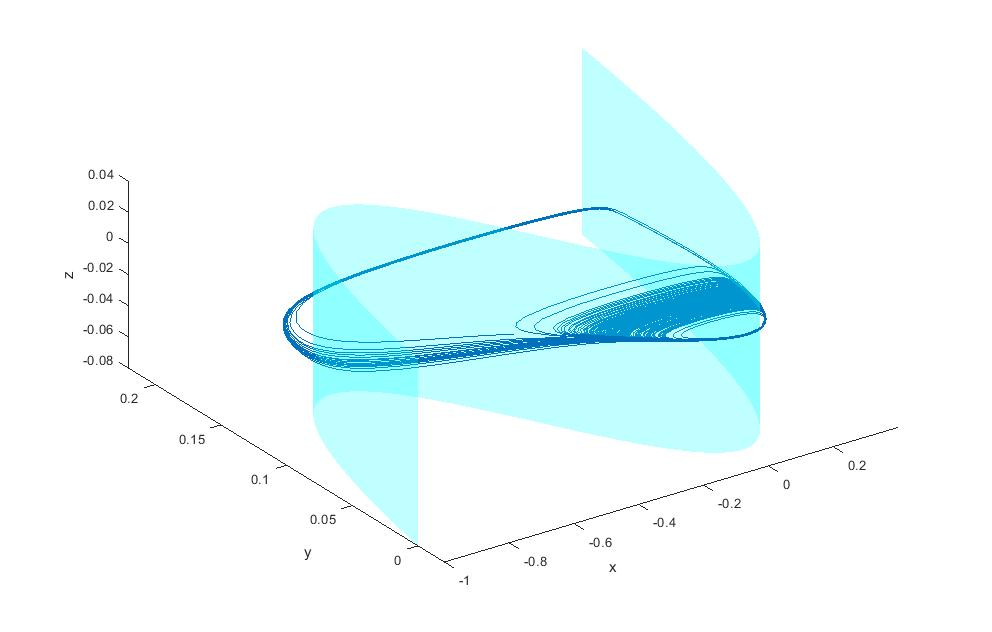
\includegraphics[width= 0.5 \textwidth]{Images/chaoticEvdp}
	\caption{Chaotic MMO orbit.}
	\label{fig: MMo3pic}
\end{figure}
\begin{figure}[h!]\centering
	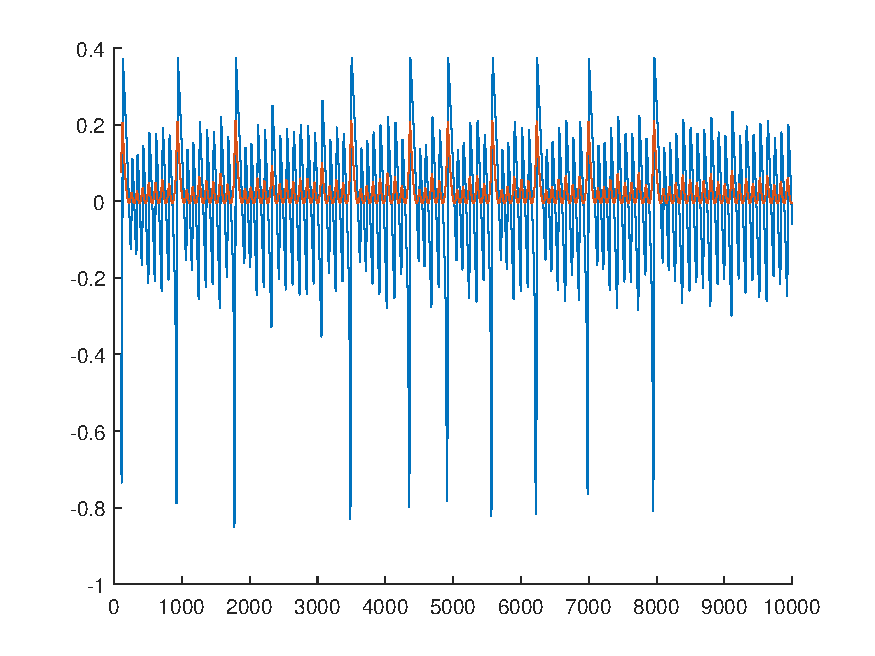
\includegraphics[width= 0.5 \textwidth]{Images/eVDPts}
	\caption{Time series for the chaotic MMO.}
	\label{fig: MMo4pic}
\end{figure}
\begin{figure}[h!]\centering
	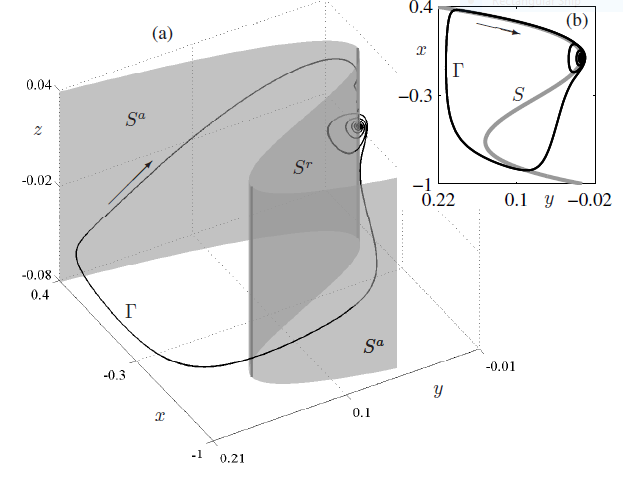
\includegraphics[width= \textwidth]{Images/MMO3}
	\caption{MMO periodic orbit for $(\nu,a,b,c)= (0.0072168,-0.3872,-0.3251,1.17,0.01)$, \citep{MMO}}
	\label{fig: MMo5pic}
\end{figure}

